\chapter{RELATED WORK}
\label{related}
The related works section is comprised of the more current projects being
developed in this problem domain, SDN.

\section{Software Defined Networking}
\label{related:sdn}
SDN provides a networking device model where the control and data planes are
decoupled from one another, where a single control plane is responsible for
distributing application execution across a set of network switches viewed as
a unified data plane instance. Applications generally operate at the control
plane level and rely on distributed platforms, such as OpenVSwitch (OVS)
\ref{ovs}, to push the logic down to the hardware level. Generally a hypervisor
sits on top of each switch and helps orchestrate the entire system.


\section{Networking Applications}
\label{related:apps}
Not all networking applications operate in the same conceptual space, that is,
they generally act as a part of a larger system. Applications can operate on a
particular traffic flow, a node within a network, or across the entire network.
% Add more to this.

\section{OpenFlow}
\label{related:of}
% Add more to this.
The OpenFlow \cite{openflow} model defines a messaging layer that the control
and, potentially distributed, data plane(s) can communicate through. This is
embodied in the OpenFlow Protocol, which specifies a set of ``instructions''
that the control and data planes must support.

\section{DPDK}
\label{related:dpdk}
Intel's Data Plane Development Kit (DPDK) \cite{dpdk} provides a framework that
allows programmers to create highly optimized data plane applications. This
platform utilizes custom drivers that provide raw access to networking devices
and computational resources. The system is tuned to natively support Intel
brand hardware and allows users to create C applications that interface with
the runtime environent. Support for higher level applications, such as C++,
require the usage of Intel's Compiler Collection (ICC), as non-portable compiler
directives are used throughout the framework and are not supported by the GNU
Compiler Collection (GCC).

\section{Open Data Plane}
\label{related:odp}
Talk about this a little bit.

\section{Open Virtual Switch}
\label{related:ovs}
Open Virtual Switch (OVS)
\begin{figure}[h]
\centering
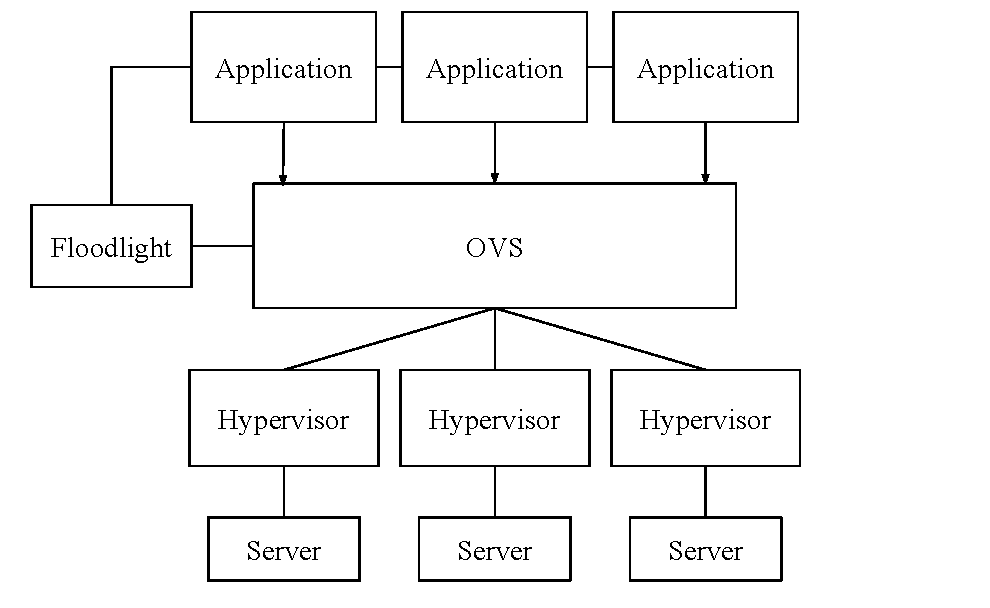
\includegraphics[scale=0.5]{ovs_arch}
\caption{The OpenVSwitch architecture.}
\label{related:ovs_arch}
\end{figure}

\section{NetASM}
\label{related:netasm}
The customized networking assembly language, NetASM \cite{netasm}, defines an
instruction set architecture (ISA) that tuned directly towards networking
programming. Instructions for modifying packet headers and state as well
as table and specialized operations are natively supported. In addition to the
networking oriented instructions the set also contains basic logical,
arithmetic, and control-flow operations. Applications written in NetASM can model
the execution environment as either a traditional Turing complete register
machine or an extended abstract machine developed by the authors.

\subsection{RISC V}
% Rewrite this.
RISC-V provides an extensible ISA, which encompasses the regular arithmetic,
logical and control-flow operations with room for a number of user-specified
instructions.

\section{Heterogenous Compute Platforms}
\label{related:hcp}
Much of the research in the domain of SDN in regards to runtime environments
encompass many of the problems found in heterogeneous computing platforms.
These issues tend to revolve around the utilization of optimized hardware
computational devices. This relates to the needs of networking programming
where a data plane is expected to be able to offload certain computation to
hardware components, such as encryption, checksums, and even packet header
processors. Below is a listing of the relevant projects in this domain that
were studied during the design and implementation of the Freeflow system.

\subsection{Heterogenous System Architecture}
\label{related:hcp:hsa}
Or HSA \cite{hsa} provides a specification for creating a heterogeneous
system architecture that supports the execution of applications across a variety
of computational resources. Interfacing with these different computing devices
requires knowledge of each devices memory model and execution semantics, and
in order to program against them the system must provide a uniform view that
each device conforms to.


\subsection{Open Compute Language}
\label{related:hcp:ocl}
Open Compute Language.

\subsection{CUDA}
\label{related:hcp:cuda}
Compute Unified Device Architecture.

\section{Frameworks}
\label{related:frameworks}
Discuss the frameworks considered.

\subsection{Seastar}
\label{related:frameworks:seastar}
Bad ass, if you've got the HW to support it.

\subsection{Libevent}
\label{related:frameworks:libevent}
Very complicated, not easy to target custom backends (dpdk).
